\chapter{Hasil dan Pembahasan}\label{ch:result}

Bab ini membahas hasil implementasi dan pengujian dari \textit{balancing} sistem \textit{reward} yang telah dirancang pada bab sebelumnya. Pembahasan mencakup rincian implementasi sistem yang meliputi pemodelan graf ekonomi, simulasi berbasis agen, dan integrasi algoritma evolusioner. Selanjutnya disajikan hasil pelaksanaan eksperimen pada model ekonomi generatif serta studi kasus menggunakan data ekonomi gim eksternal melalui \textit{game design document}, yang kemudian dianalisis untuk mengevaluasi efektivitas pendekatan yang diusulkan.

\section{Implementasi Model Sistem \textit{Reward} dan Lingkungan Simulasi}
Pada bagian ini, sistem reward dari ekonomi gim diimplementasikan menggunakan paradigma Pemrograman Berorientasi Objek (Object-Oriented Programming). Hubungan antar komponen dalam arsitektur program ini dirancang menggunakan prinsip pewarisan (inheritance) untuk memastikan modularitas. Struktur kelas tersebut secara visual direpresentasikan pada Gambar \ref{fig:arsitektur_kelas} (\nameref{fig:arsitektur_kelas}), yang memperlihatkan bagaimana kelas abstrak Node menjadi fondasi bagi seluruh entitas ekonomi dalam sistem. Sistem ekonomi dimodelkan sebagai Jaringan Logika Aliran Dinamika Skalar yang direpresentasikan melalui struktur data graf berarah (Directed Graph), di mana $G = (V, E, W)$ merupakan gabungan dari himpunan titik simpul (\textit{Nodes/Vertices}), himpunan sisi koneksi (Edges), dan matriks bobot (\textit{Weights}).

\subsection{Representasi Struktur Graf}
Struktur utama sistem dibangun di dalam kelas Graph yang bertugas sebagai pengelola seluruh daftar koneksi antar \textit{node} serta mengatur pola struktur jaringan tersebut. Kelas ini menginisialisasi arsitektur graf berdasarkan konfigurasi awal (config) yang mendefinisikan himpunan kuantitas tiap tipe titik. Dalam pembentukan graf, bobot atau nilai sisi dievaluasi menggunakan dua pendekatan:
\begin{enumerate}
    \item Bobot Deterministik: Nilai skalar riil yang merepresentasikan jumlah aliran sumber daya pasti yang dipindahkan antar simpul. Pada saat inisialisasi awal, nilai ini dapat dibangkitkan menggunakan distribusi seragam (uniform distribution).
    \item Koefisien Stokastik: Probabilitas khusus untuk simpul percabangan stokastik (rantai Markov). Untuk memastikan probabilitas transisi tetap valid, nilai probabilitas $p_i$ dibangkitkan menggunakan Parameter Distribusi Dirichlet (Distribusi Probabilitas Simplex n-dimensi) yang menjamin kriteria integral $\sum p_i = 1$ selalu terpenuhi.

\begin{figure}[htbp]
\begin{tikzpicture}[
  scale=1,
  transform shape,
  font=\sffamily\tiny,
  class/.style={
    draw=blue!50!black, thick,
    rectangle split, rectangle split parts=3,
    rectangle split part fill={blue!10, blue!5, white},
    text width=3.2cm, align=center, rounded corners=2pt
  },
  abstract/.style={
    draw=gray!70, thick, dashed,
    rectangle split, rectangle split parts=3,
    rectangle split part fill={gray!20, gray!10, white},
    text width=3.4cm, align=center, rounded corners=2pt
  },
  inherit/.style ={draw, thick,
    -{Triangle[open,fill=white,length=3.5mm,width=3mm]}},
  compose/.style ={draw, thick,
    -{Diamond[fill=black,length=3mm,width=2.2mm]}},
  associate/.style={draw, thick, -stealth}
]
 
%% ── 0a. AgentSimulator (extends Simulator) ────────────────────────
\node[class] (AgentSimulator) at (2.0,0) {
  \textbf{AgentSimulator}
  \nodepart{second}
  \begin{tabular}[t]{@{}l@{}}
    + agent : Agent \\
    + graph : Graph \\
    + monitoring : dict
  \end{tabular}
  \nodepart{third}
  \begin{tabular}[t]{@{}l@{}}
    + run(steps)
  \end{tabular}
};

%% ── 0b. Agent ─────────────────────────────────────────────────────
\node[class] (Agent) at (2.0,-3.8) {
  \textbf{Agent}
  \nodepart{second}
  \begin{tabular}[t]{@{}l@{}}
    + behavior : str
  \end{tabular}
  \nodepart{third}
  \begin{tabular}[t]{@{}l@{}}
    + play\_step(graph)
  \end{tabular}
};

%% ── 1. Simulator ──────────────────────────────────────────────────
\node[class] (Simulator) at (7.4,0) {
  \textbf{Simulator}
  \nodepart{second}
  \begin{tabular}[t]{@{}l@{}}
    + graph : Graph \\
    + monitoring : dict
  \end{tabular}
  \nodepart{third}
  \begin{tabular}[t]{@{}l@{}}
    + run(steps) \\
    + monitor() \\
    + plot\_monitor()
  \end{tabular}
};
 
%% ── 2. Graph ──────────────────────────────────────────────────────
\node[class] (Graph) at (7.4,-3.8) {
  \textbf{Graph}
  \nodepart{second}
  \begin{tabular}[t]{@{}l@{}}
    + config : dict \\
    + edge\_list : list \\
    + nodes : list \\
    + weights : list
  \end{tabular}
  \nodepart{third}
  \begin{tabular}[t]{@{}l@{}}
    + init\_nodes() \\
    + set\_edge\_weights() \\
    + simulate() \\
    + plot()
  \end{tabular}
};
 
%% ── 3. Node (Abstract) ────────────────────────────────────────────
\node[abstract] (Node) at (7.4,-8.8) {
  \textit{\textlangle\textlangle Abstract\textrangle\textrangle}\\\textbf{Node}
  \nodepart{second}
  \begin{tabular}[t]{@{}l@{}}
    + id : string \\
    + input\_edges : list \\
    + output\_edges : list
  \end{tabular}
  \nodepart{third}
  \begin{tabular}[t]{@{}l@{}}
    \textit{+ step(call\_chain)} \\
    + consume() \\
    + connect(node, value) \\
    + get\_state()
  \end{tabular}
};
 
%% ── 4. Edge ───────────────────────────────────────────────────────
\node[class] (Edge) at (2.4,-8.8) {
  \textbf{Edge}
  \nodepart{second}
  \begin{tabular}[t]{@{}l@{}}
    + value : float \\
    + node : Node
  \end{tabular}
  \nodepart{third}
  \phantom{x}
};
 
%% ── 5. Source ─────────────────────────────────────────────────────
\node[class] (Source) at (0.8,-14.0) {
  \textbf{Source}
  \nodepart{second}
  \phantom{x}
  \nodepart{third}
  \begin{tabular}[t]{@{}l@{}}
    + drop\_to(edge)
  \end{tabular}
};
 
%% ── 6. Pool ───────────────────────────────────────────────────────
\node[class] (Pool) at (4.8,-14.0) {
  \textbf{Pool}
  \nodepart{second}
  \begin{tabular}[t]{@{}l@{}}
    + pool : float
  \end{tabular}
  \nodepart{third}
  \begin{tabular}[t]{@{}l@{}}
    + consume(value) \\
    + reset()
  \end{tabular}
};
 
%% ── 7. Converter ──────────────────────────────────────────────────
\node[class] (Converter) at (9.4,-14.0) {
  \textbf{Converter}
  \nodepart{second}
  \begin{tabular}[t]{@{}l@{}}
    + is\_auto : bool \\
    + called : bool
  \end{tabular}
  \nodepart{third}
  \begin{tabular}[t]{@{}l@{}}
    + consume()
  \end{tabular}
};
 
%% ── 8. RandomGate ─────────────────────────────────────────────────
\node[class] (RandomGate) at (13.6,-14.0) {
  \textbf{RandomGate}
  \nodepart{second}
  \phantom{x}
  \nodepart{third}
  \begin{tabular}[t]{@{}l@{}}
    + consume(entity)
  \end{tabular}
};
 
%% ── 9. FixedPool ──────────────────────────────────────────────────
\node[class] (FixedPool) at (2.4,-18.8) {
  \textbf{FixedPool}
  \nodepart{second}
  \phantom{x}
  \nodepart{third}
  \begin{tabular}[t]{@{}l@{}}
    + get\_fix()
  \end{tabular}
};
 
%% ── 10. Drain ─────────────────────────────────────────────────────
\node[class] (Drain) at (7.8,-18.8) {
  \textbf{Drain}
  \nodepart{second}
  \phantom{x}
  \nodepart{third}
  \begin{tabular}[t]{@{}l@{}}
    + consume()
  \end{tabular}
};
 
%% ═══════════════ RELASI ═══════════════
 
%% AgentSimulator -▷ Simulator (pewarisan)
\draw[inherit] (AgentSimulator.east) -- (Simulator.west)
  node[midway,above=2pt,font=\tiny]{extends};

%% AgentSimulator → Agent (asosiasi kepemilikan)
\draw[associate] (AgentSimulator.south) -- (Agent.north)
  node[midway,right=2pt,font=\tiny]{menggunakan};

%% Simulator → Graph (asosiasi)
\draw[associate] (Simulator.south) -- (Graph.north)
  node[midway,right=2pt,font=\tiny]{mengoperasikan};
 
%% Graph ─◆ Node (komposisi 1..*)
\draw[compose] (Node.north) -- (Graph.south)
  node[midway,right=2pt,font=\tiny]{1..*};
 
%% Edge ─◆ Node (komposisi 0..*)
\draw[compose] (Edge.east) -- (Node.west)
  node[midway,above=2pt,font=\tiny]{0..*};
 
%% Edge.node → Node (asosiasi balik)
\draw[associate]
  (Edge.north) -- ++(0,1.5)
  -| ([xshift=-1.2cm]Node.north);
 
%% Pewarisan ke Node
\coordinate (jN) at (7.4,-11.8);
\coordinate (topLine) at (1,-11.9); % sesuaikan y

\draw[thick] (Source.north)     |- (topLine) -| (jN);
\draw[thick] (Pool.north)       |- (topLine) -| (jN);
\draw[thick] (Converter.north)  |- (topLine) -| (jN);
\draw[thick] (RandomGate.north) |- (topLine) -| (jN);
\draw[inherit] (jN) -- (Node.south);
 
%% Pewarisan ke Pool
\coordinate (jP) at (4.8,-17.1);
\draw[thick] (FixedPool.north) -- ++(0,0.6) -| (jP);
\draw[thick] (Drain.north)     -- ++(0,0.6) -| (jP);
\draw[inherit] (jP) -- (Pool.south);

\begin{scope}[shift={(10.8,0.0)}]
  % Kotak luar legenda
  \draw[draw=gray!60, rounded corners=3pt, fill=gray!5]
    (0,0) rectangle (5.8,-4.2);
 
  % Judul
  \node[font=\sffamily\small\bfseries, anchor=west] at (0.25,-0.45)
    {Legenda};
  \draw[gray!40] (0.2,-0.75) -- (5.6,-0.75);
 
  % ── Baris 1: Asosiasi ──────────────────────────────────────────
  \draw[associate] (0.3,-1.25) -- (1.6,-1.25);
  \node[font=\sffamily\tiny, anchor=west] at (1.75,-1.25)
    {Asosiasi (menggunakan)};
 
  % ── Baris 2: Komposisi ─────────────────────────────────────────
  \draw[compose] (0.3,-2.05) -- (1.6,-2.05);
  \node[font=\sffamily\tiny, anchor=west] at (1.75,-2.05)
    {Komposisi (memiliki)};
 
  % ── Baris 3: Pewarisan ─────────────────────────────────────────
  \draw[inherit] (0.3,-2.85) -- (1.6,-2.85);
  \node[font=\sffamily\tiny, anchor=west] at (1.75,-2.85)
    {Pewarisan / Inheritance};
 
  % ── Baris 7: Kelas abstrak ──────────────────────────────────────
  \draw[gray!70, thick, dashed, rounded corners=2pt]
    (0.3,-3.65) rectangle (1.6,-3.35);
  \node[font=\sffamily\tiny\itshape] at (0.95,-3.6)
    {};
  \node[font=\sffamily\tiny, anchor=west] at (1.75,-3.5)
    {Kelas abstrak};
 
\end{scope}
 
\end{tikzpicture}
\caption{Arsitektur Kelas Diagram}
\label{fig:arsitektur_kelas}
\end{figure}
    
\end{enumerate}
Graf ini juga dilengkapi dengan mekanisme normalisasi internal (scaling) untuk memverifikasi validitas properti ruang sampel probabilitas secara real-time setiap kali terjadi pembaruan atau mutasi bobot sisi selama proses simulasi berjalan.

\begin{figure}[htbp]
    \centering
    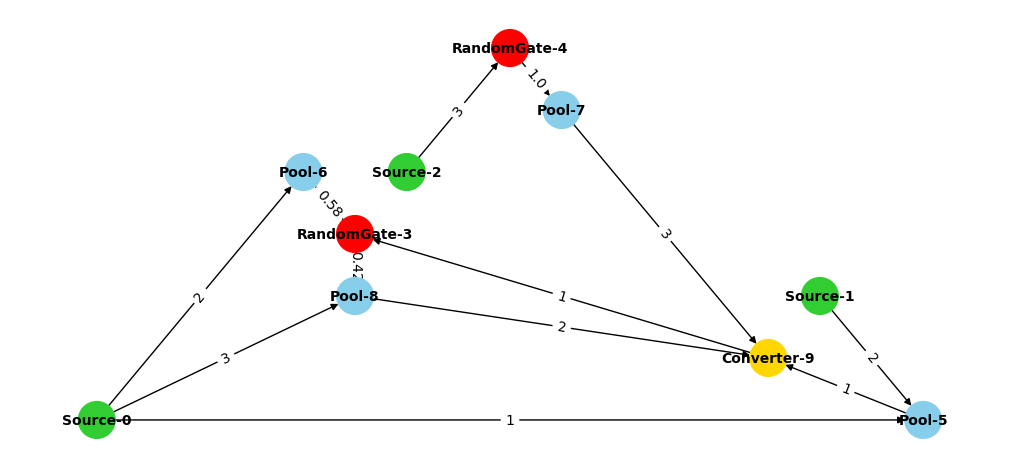
\includegraphics[width=0.7\textwidth]{tugas-akhir/assets/images/result_2.png}
    \caption{Contoh Visualisasi Struktur Graf Ekonomi Gim}
    \label{fig:initial_graph}
\end{figure}

\subsection{Implementasi \textit{Node} Ekonomi}
Setiap entitas ekonomi diwariskan (polimorfisme) dari abstraksi basis kelas \texttt{Node}. Kelas dasar ini mengatur konstrain domain fungsi input dan kodomain output, serta menerapkan hubungan antar entitas tersusun dengan benar. Evaluasi koneksi memuat Aksioma Irreflexive/Acyclic yang secara ketat menolak pembentukan loop tertutup (infinite recursion) pada simpul yang sama, sehingga arsitektur tetap berwujud \textit{Directed Acyclic Graph} (DAG).

Beberapa turunan simpul utama yang diimplementasikan meliputi:

\begin{itemize}
    \item \textit{Source},  bertindak sebagai batas titik awal ($S_0$) yang mensuplai aliran sumber daya ke dalam sistem dengan nilai in-degree sama dengan 0. Node ini mendorong transformasi nilai output maju ke subgraf selanjutnya.
    \item \textit{Pool}, simpul penyimpanan yang mengakumulasi sumber daya melalui operasi aljabar penjumlahan nilai state. Persamaan beda yang diterapkan adalah $\Delta P = P(t_{n+1}) = P(t_n) + x_{in} - x_{out}$. Terdapat variasi FixedPool yang mengimplementasikan batasan fungsi non-linier terikat $f(x) = \min(\text{pool} + x, \text{fix})$ untuk membatasi kapasitas maksimum inventaris agen.
    \item \textit{Converter}, mengeksekusi fungsi transformasi $C(x)$ yang mengubah kombinasi elemen input menjadi output baru. Simpul ini memberlakukan operator himpunan Boolean AND, di mana konversi hanya dieksekusi apabila seluruh prasyarat edge input memenuhi batas nilai $x \geq e$.
    \item \textit{RandomGate}, memodelkan percabangan aliran terbobot (weighted stochastic split). Distribusi aliran dieksekusi menggunakan percobaan probabilitas majemuk distribusi multinomial, yang mengukur vektor sampel observasi berdasarkan koefisien proporsi kejadian $P \in [0, 1]$.
    \item \textit{Drain}, Simpul sink dengan nilai out-degree sama dengan 0 yang merepresentasikan pengeluaran tak terhingga atau pembuangan variabel dari sistem persamaan diferensial.
\end{itemize}

\subsection{Implementasi Mekanisme Aliran (\textit{Edge}) dan Simulasi Waktu}
Dinamika aliran dari waktu ke waktu dieksekusi oleh mesin komputasi numerik diskret dalam kelas \texttt{Simulator} diperluas (inheritance) menjadi kelas \texttt{AgentSimulator}. Simulator ini menjalankan perulangan untuk mengevaluasi pergeseran dimensi waktu dari $t = 0$ hingga $t = n$ langkah.
% , yang dimodelkan sebagai sistem persamaan beda orde pertama:
% \[
% \mathbf{x}_{t+1} = f(\mathbf{x}_t), \quad t = 0,1,2,\dots,n-1.
% \]

Mekanisme relasi transmisi ditangani oleh objek \texttt{Edge} yang meneruskan vektor besaran dari titik $u$ ke titik tujuan $v$. 

\begin{algorithm}[h]
\caption{Simulasi Dinamika Aliran Graf Waktu Diskret}
\label{alg:graph-simulator}
\begin{algorithmic}[1]
\INPUT Graf $G = (V, E)$, jumlah langkah $n$ 
\OUTPUT Deret waktu $\mathbf{X}(t)$ untuk setiap node \textit{Pool}

\State Ekstrak himpunan node: $P$ (\textit{Pool}), $S$ (\textit{Source}), $C$ (\textit{Converter})
\State Inisialisasi struktur monitoring $\mathbf{X} \gets \emptyset$

\For{$t = 0$ hingga $n-1$}
    \For{setiap $s \in S$}
        \State $s.\text{step}()$ \Comment{Injeksi input dan propagasi dalam graf}
    \EndFor
    
    \For{setiap $p \in P$}
        \State Rekam nilai state $p$ ke $\mathbf{X}(t)$
    \EndFor
    
    \For{setiap $c \in C$}
        \State $c.\text{called} \gets \text{False}$ \Comment{Reset status evaluasi}
    \EndFor
\EndFor

\For{setiap $p \in P$}
    \State Reset state $p$
\EndFor

\State \Return $\mathbf{X}$
\end{algorithmic}
\end{algorithm}

Pada setiap iterasi waktu $t$:

\begin{enumerate}
    \item Injeksi Batas, Variabel bebas batas (\textit{boundary parameters}) dimasukkan melalui simpul \texttt{Source}.
    \item Propagasi (\textit{Forward Pass}), Nilai ditransmisikan melintasi sisi graf, mengubah state inventaris pada \texttt{Pool} dan memicu evaluasi transformasi pada \texttt{Converter} jika ketersediaan sumber daya tercukupi.
    \item Perekaman (Monitoring), Setelah propagasi selesai pada satu langkah waktu, simulator mengeksekusi metode pencatatan (snapshot) untuk merekam metrik $P(t)$ dari setiap simpul penyimpanan. Array historis ini membentuk vektor seri deret waktu $\vec{X}(t)$.
    \item Reset State, Flag status pemanggilan untuk setiap simpul perantara diatur ulang menjadi \textit{False} untuk mempersiapkan evaluasi transformasi pada interval $t+1$.
\end{enumerate}

Kumpulan matriks historis dari hasil relasi transisi ini kemudian diekspor untuk diproyeksikan sebagai grafik deret waktu, yang memvisualisasikan bagaimana aliran ekonomi berevolusi secara sekuensial.

\subsection{Implementasi  Simulasi Perilaku dan Entitas Agen}

Simulasi tidak bekerja secara pasif, melainkan dikendalikan oleh entitas otonom yang memodelkan pemain gim sungguhan menggunakan kelas \texttt{Agent}. Agen ini bertugas mengawasi simpul \texttt{Converter} yang membutuhkan pemicu manual dan tidak digerakkan murni oleh probabilitas gerbang Markov (\texttt{RandomGate}).

Logika pengambilan keputusan agen diklasifikasikan ke dalam tiga profil perilaku yang memengaruhi dinamika transisi state pada graf:

\begin{itemize}
    \item Agresif, pada model ini agen akan langsung memicu semua fungsi konversi secara maksimum pada setiap langkah waktu $t$, asalkan batas bawah prasyarat sumber daya telah terpenuhi. Model ini merepresentasikan pemain yang mengeksekusi aksi secepat mungkin tanpa menunda.
    \item Pasif, model ini mengevaluasi ketersediaan sumber daya menggunakan operasi logika Boolean AND terhadap seluruh simpul konversi manual. Agen hanya akan mengeksekusi aksi jika semua opsi konversi (\textit{skill} atau opsi \textit{crafting}) telah siap (sumber daya mencukupi dan \textit{cooldown} selesai). Jika proposisi bernilai \textit{True}, seluruh konversi dieksekusi secara bersamaan. Profil ini merepresentasikan pemain yang bermain aman dan menunggu momen optimal.
    \item Probabilistik, Pemodelan ini menggunakan pendekatan berbasis Monte-Carlo. Untuk setiap simpul konversi manual yang telah memenuhi syarat sumber daya, agen mengeksekusinya berdasarkan probabilitas sukses sebesar $p = 0.5$ (menggunakan distribusi seragam). Profil ini menyimulasikan pemain kasual yang pengambilan keputusannya tidak menentu dan probabilistik.
\end{itemize}

Integrasi antara \texttt{AgentSimulator} dan \texttt{Agent} memungkinkan algoritma optimasi nantinya tidak hanya menguji ekonomi yang berjalan secara matematis murni, tetapi juga menguji apakah ekonomi gim tersebut stabil terhadap berbagai variasi gaya bermain pemain.

\paragraph{Contoh Trace Simulasi Agen.}
Sebagai ilustrasi perbedaan perilaku antar profil agen, perhatikan contoh graf sederhana berikut. Graf memiliki satu \textit{Source} yang menginjeksikan 10 unit per langkah ke \textit{Pool\_A}. Terdapat dua \textit{Converter} manual yang keduanya menarik dari \textit{Pool\_A}: \textit{C1} membutuhkan 8 unit dan menghasilkan 12 unit ke \textit{Pool\_Out1}, serta \textit{C2} membutuhkan 10 unit dan menghasilkan 8 unit ke \textit{Pool\_Out2}. Tabel \ref{tab:agent_trace} menunjukkan dinamika sistem untuk tiga profil agen selama tiga langkah waktu.

\begin{table}[htbp]
\centering
\caption{Trace Simulasi Tiga Profil Agen pada Graf Contoh ($x = 30$)}
\label{tab:agent_trace}
\begin{adjustbox}{max width=\textwidth}
\begin{tabular}{clcccccc}
\hline
$t$ & \textbf{Profil} & \textbf{Pool\_A} & \textbf{C1 aktif?} & \textbf{C2 aktif?} & \textbf{Pool\_A akhir} & \textbf{Pool\_Out1} & \textbf{Pool\_Out2} \\
\hline
\multirow{3}{*}{0} & Aggressive & 10 & Ya (10$\geq$8)  & Tidak (10$<$10) & 2  & 12 & 0  \\
                   & Passive    & 10 & \multicolumn{2}{c}{Tidak (C2 belum siap)} & 10 & 0  & 0  \\
                   & Random     & 10 & \multicolumn{2}{c}{Masing-masing $p=0.5$} & —  & —  & —  \\
\hline
\multirow{3}{*}{1} & Aggressive & 2+10=12  & Ya (12$\geq$8) & Tidak (12$<$10) & 4  & 24 & 0  \\
                   & Passive    & 10+10=20 & \multicolumn{2}{c}{Tidak (C2 belum siap, 20$\geq$10?)} & — & — & — \\
                   & Random     & —        & \multicolumn{2}{c}{Masing-masing $p=0.5$} & — & — & — \\
\hline
\multirow{2}{*}{2} & Aggressive & 4+10=14  & Ya (14$\geq$8) & Ya (14$\geq$10) & $14{-}8{-}10=\!-4$* & 36 & 8 \\
                   & Passive    & 20+10=30 & \multicolumn{2}{c}{Ya (C1 dan C2 keduanya siap)} & $30{-}8{-}10=12$ & 12 & 8 \\
\hline
\end{tabular}
\end{adjustbox}
\end{table}

\textit{*Catatan: Pada kondisi riil, Balancer mengoptimasi bobot sehingga kasus pool negatif dihindari.}

Dari trace di atas terlihat perbedaan mendasar antar profil. Agen \textit{aggressive} langsung memicu C1 di $t=0$ begitu syaratnya terpenuhi, menghasilkan akumulasi \textit{Pool\_Out1} yang lebih cepat — namun dapat menyebabkan pool terkuras sebelum konverter lain siap. Agen \textit{passive} menunggu hingga \textit{semua} konverter siap secara bersamaan (baru $t=2$), sehingga menghasilkan output yang lebih teratur namun lebih lambat. Perbedaan pola interaksi inilah yang menciptakan variasi sinyal fitness yang diterima oleh algoritma evolusioner, mendorong eksplorasi ruang parameter yang lebih beragam dibandingkan simulasi tanpa agen.


% \section{Implementasi Simulasi Agen}
% Bagian implementasi ini menjabarkan bagaimana entitas agen dikonstruksi untuk berinteraksi di dalam lingkungan graf ekonomi. Agen, direpresentasikan dalam modul \texttt{geevo.agent\_simulation}, berinteraksi dengan tipe perilaku berbeda.

% \subsection{Pembuatan Entitas Agen}
% Kelas \texttt{Agent} menampung atribut kekayaan internal pemain (\textit{wealth}/\textit{inventory}) dan parameter preferensi yang menetapkan kecenderungannya terhadap risiko dan eksploitasi fitur dari fungsi ekonomi. Agen diinisiasi dalam variasi profil profil pemain tertentu seperti profil \textit{aggressive}, \textit{passive}, dan \textit{random}.

% \subsection{Logika Interaksi dan Kondisi \textit{State}}
% Dinamika \textit{loop} agen mensimulasikan akumulasi perolehan sumber daya pemain pada setiap langkah waktu (\textit{step}). Pada simulasi ini, \textit{auto-farming} dikontrol oleh \textit{flag} internal sementara aksi penukaran dikalkulasikan sesuai probabilitas preferensi pemain.

\section{Implementasi dan Integrasi Algoritma Evolusioner}
Algoritma evolusioner digunakan untuk secara berulang menemukan konfigurasi laju terbaik yang menyeimbangkan sistem. Komponen evolusi dienkapsulasi pada kelas \texttt{Balancer}.

\subsection{Representasi Kromosom Konfigurasi \textit{Reward}}
Vektor numerik merepresentasikan bobot probabilitas, laju \textit{source}, serta harga komoditas (laju \textit{sink}/\textit{drain}). Vektor ini bermutasi dan disilangkan pada proses reproduksi algoritma penyeimbangan.

\subsection{Fungsi \textit{Fitness}}
Nilai \textit{fitness} dievaluasi dari performa ekonomi melalui simulasi singkat dengan kondisi terukur. Keseimbangan (fitness tertinggi) didefinisikan sebagai tingkat stabilitas terbaik di mana sistem terhindar dari inflasi maupun krisis sumber daya ekstrem.

Dua fungsi fitness diimplementasikan dalam penelitian ini untuk membandingkan efektivitas pendekatan evaluasi yang berbeda:

\begin{enumerate}
    \item \textbf{Fungsi Objektif 3 (obj3)}, merupakan fungsi proporsional yang diadaptasi dari kerangka GEEvo \citep{Rupp_2024}. Nilai fitness diukur berdasarkan rasio proporsional antara nilai aktual pool $s_t$ pada langkah waktu akhir dan nilai target $x$:
    \[
        f_3(s_t, x) = \frac{\min(s_t,\; x)}{\max(s_t,\; x)} \longrightarrow \max \approx 1.0
    \]
    Sistem dinyatakan seimbang (\textit{balanced}) apabila nilai fitness mencapai ambang $f_3 \geq 1 - \alpha$.

    \item \textbf{Fungsi Objektif 4 (obj4)}, merupakan kontribusi penelitian ini sebagai varian obj3 dengan mekanisme \textit{tolerance-threshold}. Fungsi ini memberikan nilai fitness sempurna ($f = 1.0$) apabila nilai aktual berada dalam toleransi $\alpha$ terhadap target, dan kembali ke formula proporsional apabila di luar batas tersebut:
    \[
        f_4(s_t, x) =
        \begin{cases}
            1.0 & \text{jika } |x - s_t| \leq \alpha \cdot x \\[4pt]
            \dfrac{\min(s_t,\; x)}{\max(s_t,\; x)} & \text{sebaliknya}
        \end{cases}
    \]
    Modifikasi ini menciptakan \textit{reward plateau} di sekitar nilai target, sehingga memberikan gradien sinyal yang lebih informatif bagi algoritma evolusioner untuk konvergen lebih cepat.
\end{enumerate}

Fitness dievaluasi melalui $n_{\text{sim}} = 10$ simulasi Monte-Carlo per individu untuk mereduksi bias variansi akibat perilaku agen yang stokastik. Nilai fitness akhir merupakan rata-rata dari seluruh simulasi tersebut.

Sebagai ilustrasi perbedaan konkret antara obj3 dan obj4, perhatikan contoh berikut. Misalkan target $x = 30$, $\alpha = 0.05$, sehingga toleransi obj4 adalah $\alpha \cdot x = 0.05 \times 30 = 1.5$ dan ambang keseimbangan obj3 adalah $1 - \alpha = 0.95$.

\begin{table}[htbp]
\centering
\caption{Perbandingan Nilai obj3 dan obj4 untuk Berbagai $s_t$ ($x = 30,\ \alpha = 0.05$)}
\label{tab:obj_example}
\begin{tabular}{ccccc}
\hline
\textbf{Nilai Pool} $s_t$ & \textbf{$f_3$} & \textbf{$f_4$} & \textbf{Seimbang (obj3, $\geq 0.95$)} & \textbf{Seimbang (obj4, $|30{-}s_t| \leq 1.5$)} \\
\hline
10.0 & 0.333 & 0.333 & Tidak & Tidak \\
25.0 & 0.833 & 0.833 & Tidak & Tidak \\
28.0 & 0.933 & 0.933 & Tidak & Tidak \\
28.5 & 0.950 & \textbf{1.000} & Ya    & Ya    \\
29.0 & 0.967 & \textbf{1.000} & Ya    & Ya    \\
30.0 & 1.000 & \textbf{1.000} & Ya    & Ya    \\
31.0 & 0.968 & \textbf{1.000} & Ya    & Ya    \\
31.5 & 0.952 & \textbf{1.000} & Ya    & Ya    \\
32.0 & 0.938 & 0.938 & Tidak & Tidak \\
35.0 & 0.857 & 0.857 & Tidak & Tidak \\
\hline
\end{tabular}
\end{table}

Tabel \ref{tab:obj_example} menunjukkan perbedaan kritis antara kedua fungsi. Untuk $s_t = 29$ misalnya, obj3 menghasilkan fitness $29/30 = 0.967$, sementara obj4 memberikan $1.000$ karena $|30 - 29| = 1 \leq 1.5$. Keduanya menyatakan kondisi \textit{balanced}, tetapi sinyal yang dikirimkan berbeda: obj4 memberikan sinyal tegas ``sudah optimal'' sehingga algoritma dapat berhenti lebih awal. Sebaliknya, untuk $s_t = 32$ di mana pool \textit{melebihi} target, obj3 memberi 0.938 (tidak seimbang) dan obj4 juga memberi 0.938 karena $|30 - 32| = 2 > 1.5$. Zona keseimbangan obj4 bersifat simetris terhadap target (28.5 hingga 31.5), memberikan tekanan seleksi yang setara untuk pool yang kekurangan maupun kelebihan sumber daya.

Kurva pencarian penyeimbangan model utama ditunjukkan pada pencarian \texttt{EvoGraphGenerator} di Gambar \ref{fig:egg_fitness}.

\begin{figure}[htbp]
    \centering
    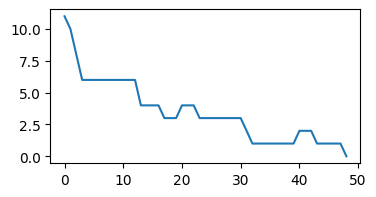
\includegraphics[width=0.6\textwidth]{tugas-akhir/assets/images/result_1.png}
    \caption{Historis Evaluasi \textit{Fitness} Algoritma Evolusi Generatif}
    \label{fig:egg_fitness}
\end{figure}

\section{Pelaksanaan Uji Coba dan Studi Kasus}
% Pelaksanaan dilakukan dengan menyimulasikan iterasi pada beberapa profil perilaku agen dan dengan desain graf sebelum maupun sesudah penerapan optimasi algoritma.

\subsection{Deskripsi Data \textit{Game Design Document}}

Pengujian pada data eksternal dilakukan menggunakan dua \textit{Game Design Document} (GDD) nyata yang dipilih berdasarkan perbedaan kompleksitas sistem ekonominya. Pemilihan dua GDD yang kontras bertujuan untuk menguji kemampuan generalisasi model terhadap topologi ekonomi yang beragam.

\begin{enumerate}
    \item \textbf{MMORPG Game Design Document} (\texttt{MMORPG\_GameDesign\_v27.pdf}), merupakan dokumen desain untuk gim \textit{massively multiplayer online role-playing game} dengan sistem ekonomi kompleks yang mencakup mekanisme pengumpulan mata uang emas, penyimpanan sumber daya bertingkat, \textit{crafting}, \textit{upgrading}, dan distribusi probabilistik hadiah. Proses ekstraksi kata kunci menghasilkan konfigurasi node $\{$\textit{Source}: 2, \textit{RandomGate}: 3, \textit{Pool}: 5, \textit{Converter}: 3$\}$, menghasilkan total 13 node yang merepresentasikan kompleksitas ekonomi kelas MMORPG.

    \item \textbf{VHS Horror Game Design Document} (\texttt{VHS-Horror-Game-Design-Document.pdf}), merupakan dokumen desain untuk gim \textit{survival horror} dengan sistem ekonomi yang lebih sederhana, berfokus pada inventori terbatas dan mekanisme bertahan hidup. Ekstraksi menghasilkan konfigurasi node $\{$\textit{Source}: 1, \textit{RandomGate}: 2, \textit{Pool}: 3, \textit{Converter}: 1$\}$, menghasilkan total 7 node yang mencerminkan minimnya sumber daya dalam gim bertipe \textit{survival}.
\end{enumerate}

Untuk setiap dataset GDD, sebanyak $n = 10$ graf ekonomi dibangkitkan menggunakan \texttt{EvolutionaryGraphGeneration} (EGG) berdasarkan konfigurasi yang diekstrak. Seluruh eksperimen pada dataset GDD menggunakan kondisi TA penuh (Kondisi C: simulasi agen + obj4) sebagai representasi kontribusi akhir penelitian ini.

\subsection{Mekanisme Penerjemahan GDD Menjadi Bentuk Graf}

Penerjemahan GDD menjadi konfigurasi graf ekonomi dilakukan oleh modul \texttt{GDDExtractor} yang dikembangkan sebagai kontribusi penelitian ini. Proses penerjemahan berlangsung dalam tiga tahap:

\begin{enumerate}
    \item \textbf{Ekstraksi Teks PDF}, modul membaca teks seluruh halaman dokumen GDD menggunakan pustaka \textit{PyMuPDF} atau \textit{PyPDF2} sebagai alternatif. Teks seluruh dokumen diproses dalam bentuk huruf kecil (\textit{lowercase}) untuk normalisasi pencocokan kata kunci.

    \item \textbf{Pemetaan Kata Kunci (\textit{Keyword Matching})}, setiap tipe node GEEvo dipetakan ke satu himpunan kata kunci yang merepresentasikan konsep ekonomi relevan dalam bahasa natural. Frekuensi kemunculan kata kunci di seluruh dokumen dihitung untuk setiap tipe node, sebagaimana dirinci pada Tabel \ref{tab:keyword_map}.

    \item \textbf{Konversi Proporsional ke Konfigurasi Node}, hasil perhitungan frekuensi dikonversi secara proporsional menjadi jumlah node setiap tipe. Setiap tipe node dijamin mendapat minimal satu node, dan total node dibatasi sesuai parameter \texttt{max\_nodes}. Konfigurasi yang dihasilkan selanjutnya digunakan sebagai masukan EGG untuk membangkitkan topologi graf.
\end{enumerate}

\begin{table}[htbp]
\centering
\caption{Pemetaan Kata Kunci ke Tipe Node GEEvo}
\label{tab:keyword_map}
\begin{tabular}{ll}
\hline
\textbf{Tipe Node} & \textbf{Contoh Kata Kunci} \\
\hline
\textit{Source}     & drop, reward, quest, loot, gather, generate, spawn, earn, produce \\
\textit{Pool}       & gold, currency, resource, inventory, wallet, balance, mana, xp, health \\
\textit{Converter}  & shop, crafting, trade, market, upgrade, buy, sell, convert, forge \\
\textit{RandomGate} & chance, luck, rng, random, gamble, gacha, dice, drop rate, loot table \\
\hline
\end{tabular}
\end{table}

\begin{algorithm}[h]
\caption{Ekstraksi Konfigurasi GEEvo dari GDD}
\label{alg:gdd-extractor}
\begin{algorithmic}[1]
\INPUT Jalur file GDD $P_{pdf}$, jumlah maksimum node $N_{max}$
\OUTPUT Konfigurasi node $C = \{$\textit{Source}, \textit{Pool}, \textit{Converter}, \textit{RandomGate}$\}$

\State Baca teks seluruh halaman GDD: $T \gets \text{read\_pdf}(P_{pdf})$
\For{setiap tipe node $k \in \{$\textit{Source, Pool, Converter, RandomGate}$\}$}
    \State $w_k \gets \sum_{\text{keyword} \in K_k} \text{count}(\text{keyword},\; T)$
\EndFor
\If{$\sum_k w_k = 0$}
    \State \Return konfigurasi \textit{fallback} default $\{$S:2, P:4, C:2, RG:1$\}$
\EndIf
\State Distribusikan $N_{max}$ node secara proporsional berdasarkan $w_k$
\State Jamin minimal 1 node per tipe
\State \Return konfigurasi $C$
\end{algorithmic}
\end{algorithm}

\subsection{Skenario Uji Coba Dinamika Graf Generatif}

Uji coba dilakukan dalam dua skenario utama yang bertujuan mengevaluasi efektivitas pendekatan dari sudut pandang berbeda:

\begin{enumerate}
    \item \textbf{Skenario Generatif (Abstrak)}, sebanyak $n = 30$ graf ekonomi dibangkitkan secara generatif menggunakan konfigurasi abstrak ($\textit{Source}: 3, \textit{RandomGate}: 2, \textit{Pool}: 4, \textit{Converter}: 1$). Skenario ini mengevaluasi kemampuan dasar sistem penyeimbangan pada topologi yang dikontrol. Sebagai pelengkap, dilakukan juga perbandingan tiga kondisi evaluasi (A, B, C) pada $n = 194$ graf abstrak dengan konfigurasi yang sama untuk mengisolasi kontribusi masing-masing komponen yang diusulkan.

    \item \textbf{Skenario GDD (Data Nyata)}, menggunakan dua GDD nyata (MMORPG dan VHS) sebagai masukan eksternal. Masing-masing menghasilkan $n = 10$ graf yang topologinya diekstrak otomatis dari konten dokumen, kemudian diseimbangkan menggunakan kondisi penelitian penuh (Kondisi C).
\end{enumerate}

Tiga kondisi evaluasi yang dibandingkan dalam penelitian ini adalah:
\begin{itemize}
    \item \textbf{Kondisi A} : tanpa agen (simulasi pasif), fungsi fitness obj3 (baseline replikasi paper)
    \item \textbf{Kondisi B} : dengan agen (\textit{aggressive}, \textit{passive}, \textit{random}), fungsi fitness obj3 (isolasi dampak agen)
    \item \textbf{Kondisi C} : dengan agen, fungsi fitness obj4 (kondisi penelitian penuh, kontribusi utama)
\end{itemize}

Gambar \ref{fig:unbalanced} dan Gambar \ref{fig:balanced_graph} menunjukkan perbandingan visual struktur aliran sumber daya sebelum dan sesudah proses penyeimbangan pada salah satu contoh graf generatif.

\begin{figure}[htbp]
    \centering
    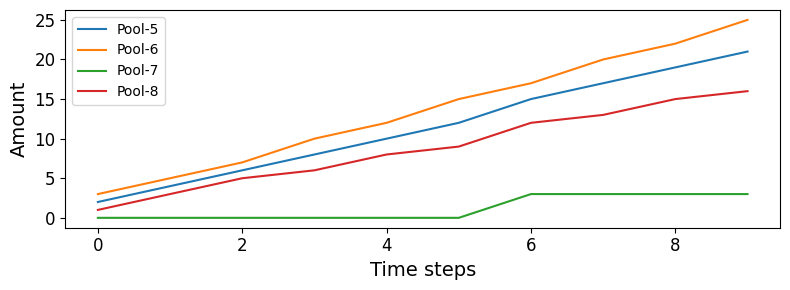
\includegraphics[width=0.7\textwidth]{tugas-akhir/assets/images/result_3.png}
    \caption{Simulasi Interaksi Agen pada Kondisi Graf Belum Seimbang}
    \label{fig:unbalanced}
\end{figure}

\begin{figure}[htbp]
    \centering
    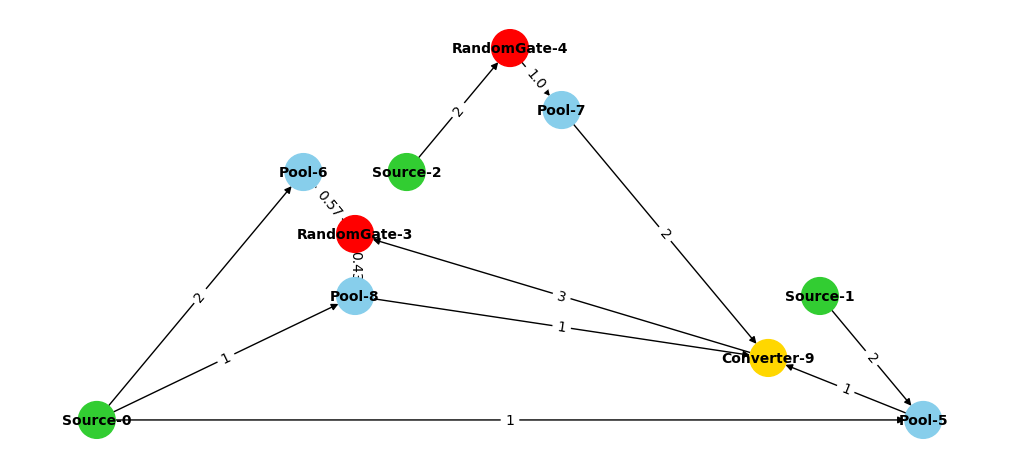
\includegraphics[width=0.7\textwidth]{tugas-akhir/assets/images/result_5.png}
    \caption{Visualisasi Graf Ekonomi Generatif dengan Bobot \textit{Reward} Optimal}
    \label{fig:balanced_graph}
\end{figure}

\section{Analisis Hasil}
Analisis ini membandingkan fluktuasi pasokan sistem serta evaluasi \textit{fitness} algoritma secara holistik dari model \textit{baseline} menuju model yang telah dioptimasi algoritma \textit{reward balancing}.

\subsection{Kestabilan Sumber Daya pada Ekonomi Gim}
Memperhatikan performa awal dari Gambar \ref{fig:unbalanced}, perbandingan stabilitas diuji simulasi pada graf berbobot optimal. Gambar \ref{fig:balanced_sim} menunjukkan bahwa model telah berhasil mencegah akumulasi eksponensial maupun penipisan sumber daya selama iterasi agen, dan menjaga ekonomi di kondisi stasioner dinamis.

\begin{figure}[htbp]
    \centering
    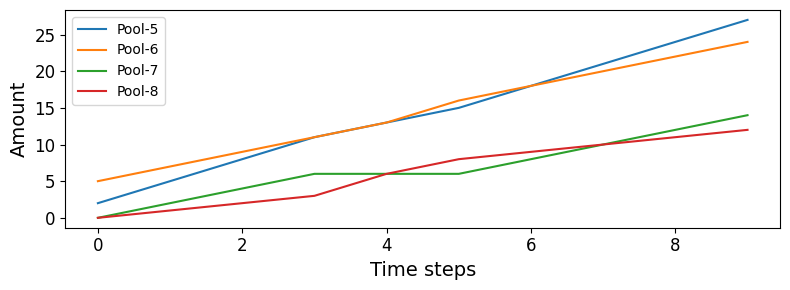
\includegraphics[width=0.7\textwidth]{tugas-akhir/assets/images/result_6.png}
    \caption{Kestabilan Dinamika Volume Pool setelah Optimasi Konfigurasi Harga}
    \label{fig:balanced_sim}
\end{figure}

\subsection{Analisis Dinamika dan Perilaku Agen}
Uji coba menggunakan agen \textit{aggressive}, \textit{passive}, dan \textit{random} memvalidasi bahwa sistem teroptimasi memberikan batas kewajaran ekonomi lintas jenis pemain, terhimpun pada Gambar \ref{fig:agent_behaviors}. Perbedaan kecuraman aliran sumber daya yang dapat dicapai menunjukkan kerentanan spesifik tiap tipe dapat dieksplorasi pemain pada area \textit{Converter} \textit{manual} tanpa mendisrupsi ekuilibrium seluruh ekosistem gim.

\begin{figure}[htbp]
    \centering
    \begin{minipage}{0.48\textwidth}
        \centering
        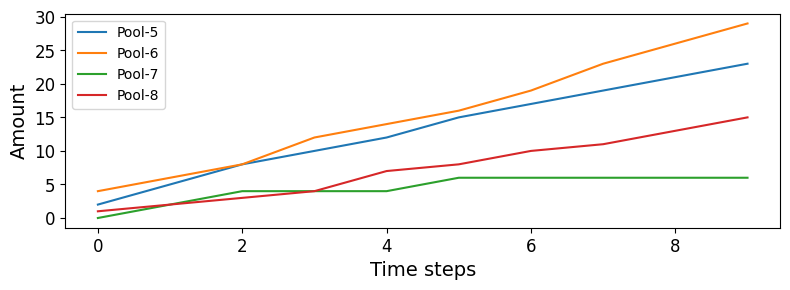
\includegraphics[width=\textwidth]{tugas-akhir/assets/images/result_7.png}
        \subcaption{Simulasi Agen \textit{Aggressive}}
    \end{minipage}
    \begin{minipage}{0.48\textwidth}
        \centering
        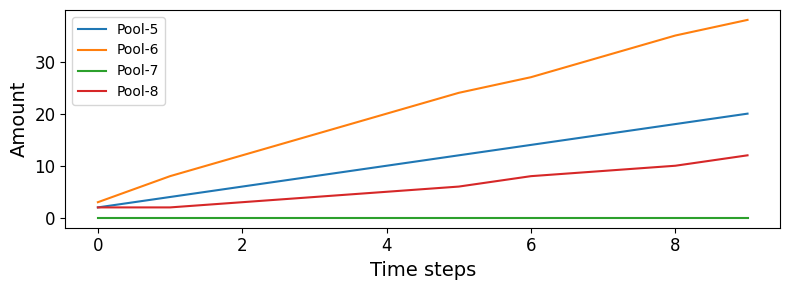
\includegraphics[width=\textwidth]{tugas-akhir/assets/images/result_8.png}
        \subcaption{Simulasi Agen \textit{Passive}}
    \end{minipage}
    \caption{Perbandingan Dinamika Interaksi Profil Agen Berbeda \textit{Post-Balance}}
    \label{fig:agent_behaviors}
\end{figure}

\subsection{Evaluasi Kinerja Algoritma Evolusioner (Konvergensi \textit{Fitness})}
Algoritma utama (\texttt{Balancer}) terbukti berhasil menemukan titik batas maksimum (penurunan beban deviasi hingga konvergen) di mana bobot \textit{sink} dan probabilitas dapat beradaptasi secara heuristik. Hal ini tergambar jelas pada kenaikan performa historis konvergensi populasi parameter \textit{balancer} dari simulasi menuju optimasi maksimal (Gambar \ref{fig:balancer_monitor}).

\begin{figure}[htbp]
    \centering
    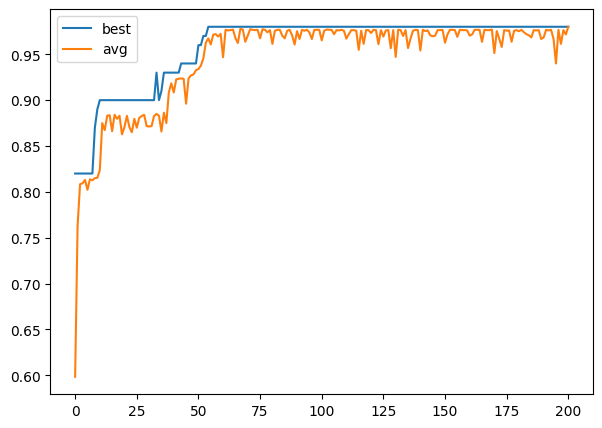
\includegraphics[width=0.6\textwidth]{tugas-akhir/assets/images/result_4.png}
    \caption{Kurva Konvergensi Metrik Evaluasi Optimasi \textit{Balancer}}
    \label{fig:balancer_monitor}
\end{figure}

\subsection{Evaluasi Komparatif Tiga Kondisi Eksperimen}
\label{subsec:abc_comparison}

Untuk mengisolasi kontribusi masing-masing komponen yang diusulkan, dilakukan evaluasi komparatif terhadap tiga kondisi pada $n = 194$ graf abstrak dengan tiga nilai parameter $\alpha$. Hasil perbandingan lengkap ditunjukkan pada Tabel \ref{tab:abc_full}.

\begin{table}[htbp]
\centering
\caption{Hasil Lengkap Ketiga Kondisi Evaluasi ($n=194$ Graf Abstrak)}
\label{tab:abc_full}
\begin{tabular}{llccccc}
\hline
\textbf{Kondisi} & $\alpha$ & \textbf{Bal.\%} & \textbf{Init.Bal.\%} & \textbf{Impr.\%} & \textbf{Std Dev} & \textbf{Med.Gen} \\
\hline
A: Tanpa Agen + obj3 & 0.05 & 48.97 & 3.09 & 78.35 & 0.293 & 500 \\
A: Tanpa Agen + obj3 & 0.01 & 14.95 & 1.03 & 82.99 & 0.245 & 500 \\
A: Tanpa Agen + obj3 & 0.00 &  4.64 & 0.52 & 80.41 & 0.231 & 500 \\
\hline
B: Agen + obj3       & 0.05 & 46.39 & 3.09 & 81.44 & 0.243 & 500 \\
B: Agen + obj3       & 0.01 & 12.37 & 1.55 & 86.60 & 0.192 & 500 \\
B: Agen + obj3       & 0.00 &  3.09 & 0.00 & 84.54 & 0.230 & 500 \\
\hline
\textbf{C: Agen + obj4 (TA)} & \textbf{0.05} & \textbf{54.64} & \textbf{3.09} & \textbf{87.11} & \textbf{0.240} & \textbf{8} \\
C: Agen + obj4 (TA)  & 0.01 & 15.46 & 0.52 & 84.54 & 0.235 & 500 \\
C: Agen + obj4 (TA)  & 0.00 &  3.09 & 0.00 & 84.54 & 0.230 & 500 \\
\hline
\end{tabular}
\end{table}

Tabel \ref{tab:abc_full} mengungkap dua temuan kunci tentang kontribusi masing-masing komponen:

\paragraph{Dampak Simulasi Agen (Kondisi B vs. A).}
Hasil pengujian menunjukkan bahwa Kondisi B secara konsisten mengungguli Kondisi A pada metrik \textit{Improved \%} di seluruh nilai $\alpha$. Peningkatan performa tercatat sebesar $3{,}09\%$ pada $\alpha=0{,}05$, $3{,}61\%$ pada $\alpha=0{,}01$, dan mencapai $4{,}13\%$ pada $\alpha=0{,}0$. Selain itu, nilai \textit{Fitness Std Dev} pada Kondisi B senantiasa lebih rendah dibandingkan Kondisi A, dengan perbedaan paling signifikan terlihat pada $\alpha=0{,}01$ ($0{,}192$ vs. $0{,}245$). Hal ini mengindikasikan bahwa penggunaan agen menghasilkan proses pencarian yang lebih stabil dan konsisten di berbagai topologi graf. Kontribusi agen ini terbukti bersifat robust dan stabil, terlepas dari tingkat keketatan ambang batas (\textit{threshold}) yang diterapkan.

\paragraph{Dampak \textit{obj4} (Kondisi C vs. B).}
Berbeda dengan simulasi agen, keunggulan fungsi \textit{obj4} ditemukan bersifat kondisional terhadap nilai $\alpha$. Keuntungan penggunaan \textit{obj4} terkonsentrasi pada $\alpha = 0{,}05$, yang ditandai dengan kenaikan \textit{Balanced \%} sebesar $8{,}25\%$, \textit{Improved \%} sebesar $5{,}67\%$, serta penurunan \textit{Median Generation} yang drastis dari $500$ menjadi $8$ generasi. Namun, pada $\alpha = 0{,}01$ dan $\alpha = 0{,}0$, hasil antara Kondisi B dan C cenderung identik. Fenomena ini terjadi karena rentang toleransi \textit{obj4} menjadi sangat sempit ($0{,}01 \times 30 = 0{,}3$ unit), sehingga mekanisme \textit{plateau} tidak lagi teraktivasi dan fungsi \textit{obj4} berperilaku ekuivalen dengan \textit{obj3}. Pola tersebut menunjukkan bahwa \textit{obj4} memberikan manfaat nyata pada \textit{threshold} yang lebih longgar, sementara pada \textit{threshold} ketat, gradien seleksi dari kedua fungsi tersebut menjadi serupa.

Gambar \ref{fig:convergence_abc} menunjukkan perbandingan kurva konvergensi dari ketiga kondisi tersebut.

\begin{figure}[htbp]
    \centering
    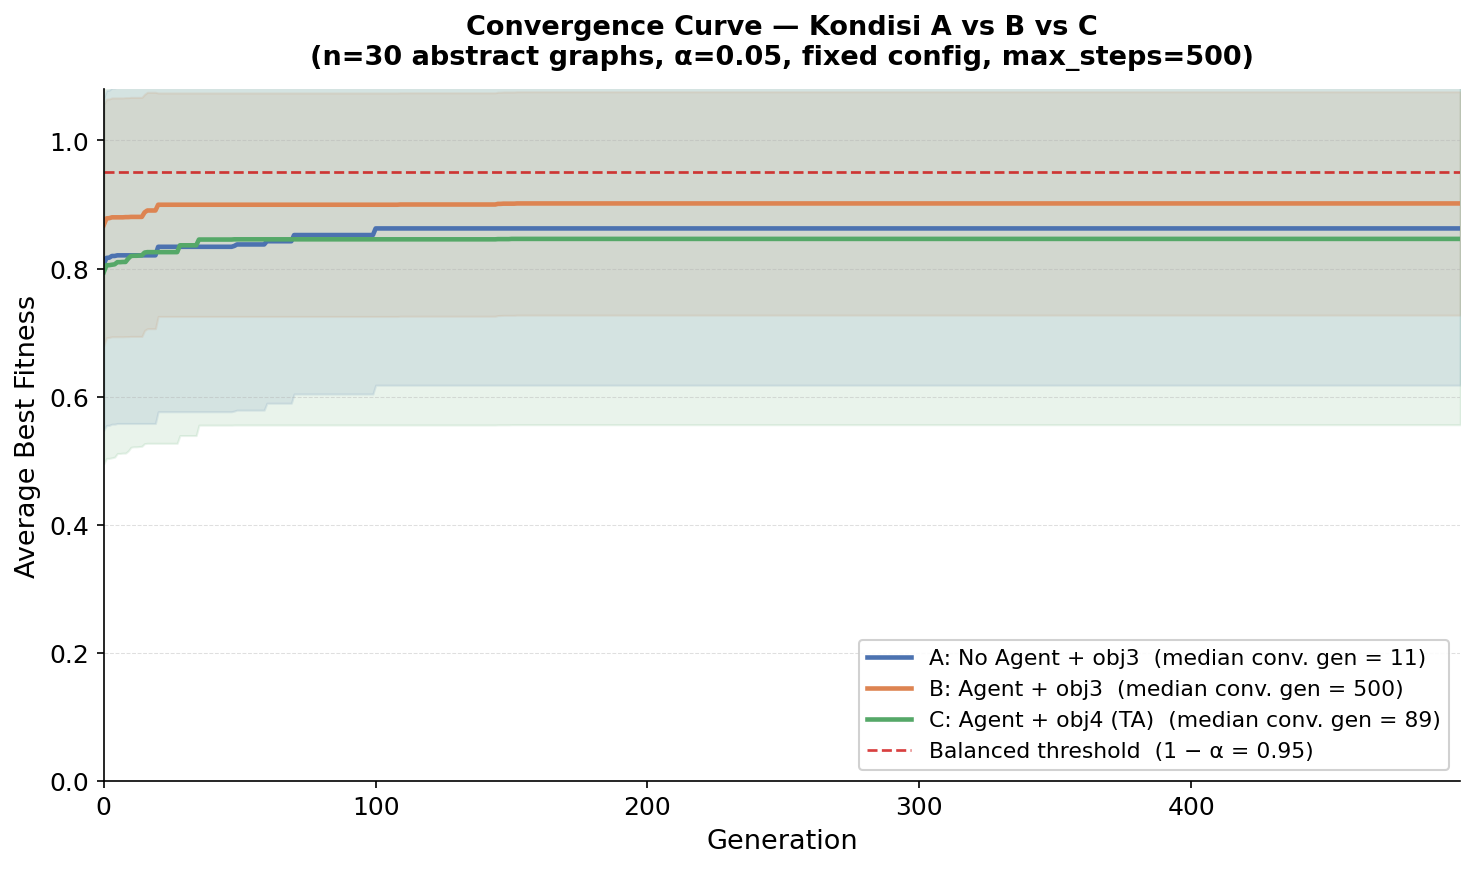
\includegraphics[width=0.85\textwidth]{tugas-akhir/assets/images/convergence_abc.png}
    \caption{Perbandingan Kurva Konvergensi \textit{Fitness} Ketiga Kondisi Evaluasi ($n=194$, $\alpha=0.05$)}
    \label{fig:convergence_abc}
\end{figure}

\subsection{Evaluasi Penyeimbangan pada Dataset GDD}
\label{subsec:gdd_results}

Evaluasi pada dataset GDD nyata dilakukan menggunakan kondisi TA penuh (Kondisi C). Tabel \ref{tab:mmorpg_results} dan Tabel \ref{tab:vhs_results} merangkum hasil penyeimbangan pada kedua dataset di berbagai nilai $\alpha$.

\begin{table}[htbp]
\centering
\caption{Hasil Evaluasi pada Dataset MMORPG GDD ($n=10$, Kondisi C)}
\label{tab:mmorpg_results}
\begin{tabular}{lccccc}
\hline
$\alpha$ & \textbf{Balanced \%} & \textbf{Initial Bal. \%} & \textbf{Improved \%} & \textbf{Median Gen} & \textbf{Exec Time (s)} \\
\hline
0.05 & 50.0\%  & 10.0\% & 70.0\%  & 251.0 & 3.609  \\
0.01 & 0.0\%   & 0.0\%  & 60.0\%  & 500.0 & 40.778 \\
0.0  & 10.0\%  & 0.0\%  & 80.0\%  & 500.0 & 54.733 \\
\hline
\end{tabular}
\end{table}

\begin{table}[htbp]
\centering
\caption{Hasil Evaluasi pada Dataset VHS Horror GDD ($n=10$, Kondisi C)}
\label{tab:vhs_results}
\begin{tabular}{lccccc}
\hline
$\alpha$ & \textbf{Balanced \%} & \textbf{Initial Bal. \%} & \textbf{Improved \%} & \textbf{Median Gen} & \textbf{Exec Time (s)} \\
\hline
0.05 & 30.0\% & 0.0\% & 100.0\% & 500.0 & 18.004 \\
0.01 & 20.0\% & 0.0\% & 100.0\% & 500.0 & 3.575  \\
0.0  & 0.0\%  & 0.0\% & 90.0\%  & 500.0 & 5.084  \\
\hline
\end{tabular}
\end{table}

\textbf{Dataset MMORPG.} Pada $\alpha = 0.05$, setengah dari total graf (50\%) berhasil mencapai kondisi seimbang, namun dengan median generasi 251 — jauh lebih lambat dibanding dataset abstrak (2.5 generasi). Perbedaan ini mencerminkan kompleksitas topologi MMORPG yang lebih tinggi (13 node, 3 \textit{Converter}) yang memperluas ruang pencarian algoritma. Sebesar 70\% graf tetap mengalami perbaikan (\textit{Improved}), menunjukkan bahwa algoritma efektif menemukan konfigurasi yang lebih baik meskipun tidak selalu mencapai ambang keseimbangan penuh. Kurva konvergensi dataset MMORPG ditunjukkan pada Gambar \ref{fig:konvergensi_mmorpg}.

\begin{figure}[htbp]
    \centering
    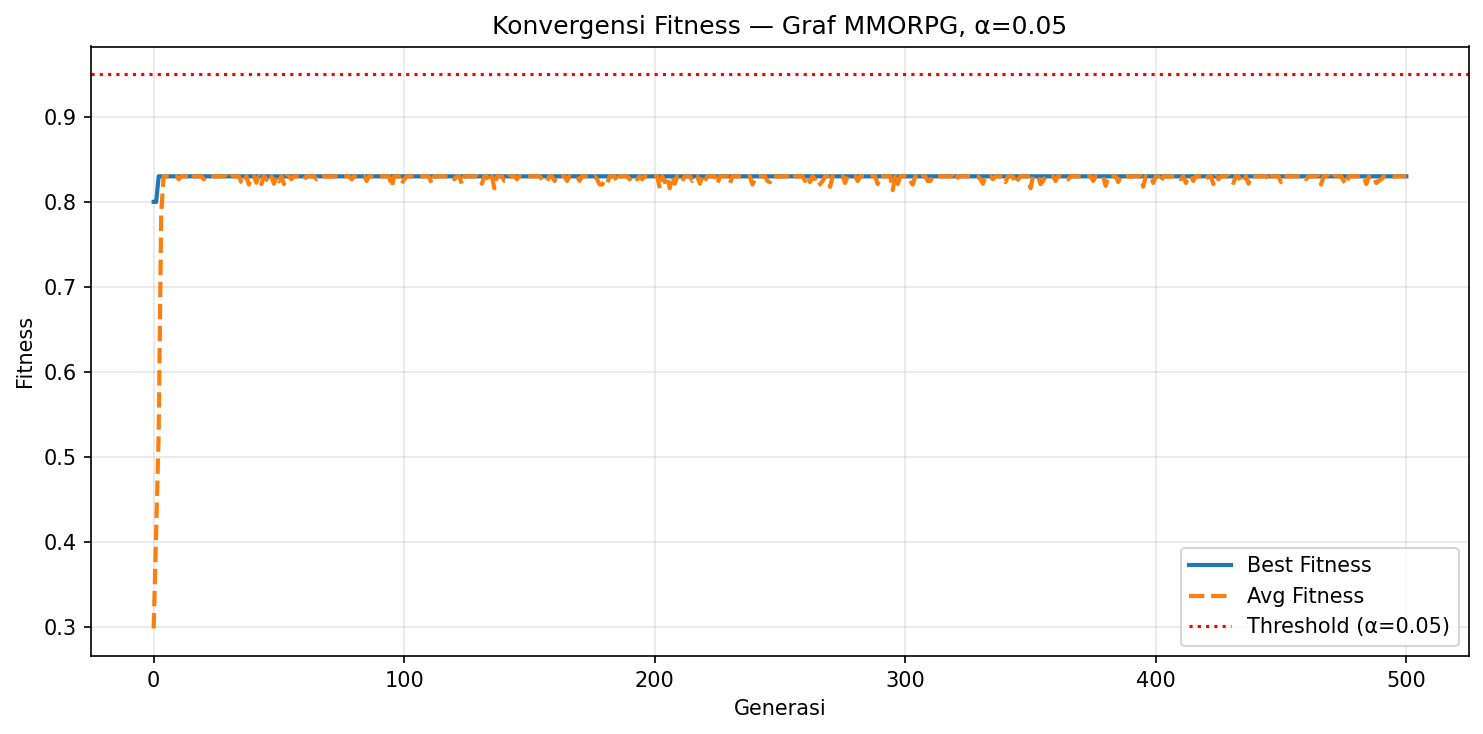
\includegraphics[width=0.75\textwidth]{tugas-akhir/assets/images/plot_konvergensi_mmorpg.png}
    \caption{Kurva Konvergensi \textit{Fitness} pada Dataset MMORPG GDD}
    \label{fig:konvergensi_mmorpg}
\end{figure}

\textbf{Dataset VHS Horror.} Dataset VHS menunjukkan pola yang berbeda: meskipun \textit{Balanced \%} relatif rendah (30\% pada $\alpha = 0.05$), tingkat \textit{Improved \%} mencapai 100\% pada dua nilai $\alpha$ (0.05 dan 0.01), artinya seluruh graf mengalami perbaikan dari kondisi awalnya. Hal ini mengindikasikan bahwa topologi VHS yang lebih sederhana (7 node) lebih mudah diperbaiki secara relatif, meskipun ambang keseimbangan tetap sulit dicapai karena tidak ada satu pun graf yang seimbang pada kondisi awal (\textit{Initial Balanced} = 0\%). \textit{Fitness Std Dev} yang sangat rendah (0.0507 pada $\alpha = 0.05$) juga menunjukkan konsistensi hasil yang tinggi pada dataset ini.

Analisis distribusi per tipe agen pada dataset abstrak ($\alpha = 0.05$) disajikan pada Tabel \ref{tab:per_agent} dan Gambar \ref{fig:per_agent_plot}.

\begin{table}[htbp]
\centering
\caption{Perbandingan Hasil per Profil Agen pada Dataset Abstrak ($n=30$, $\alpha=0.05$, Kondisi C)}
\label{tab:per_agent}
\begin{tabular}{lccc}
\hline
\textbf{Profil Agen} & \textbf{Balanced \%} & \textbf{Improved \%} & \textbf{Median Gen} \\
\hline
\textit{Aggressive} & 63.33\% & 83.33\% & 3.0 \\
\textit{Passive}    & 60.00\% & 83.33\% & 6.5 \\
\textit{Random}     & 56.67\% & 73.33\% & 6.5 \\
\hline
\end{tabular}
\end{table}

\begin{figure}[htbp]
    \centering
    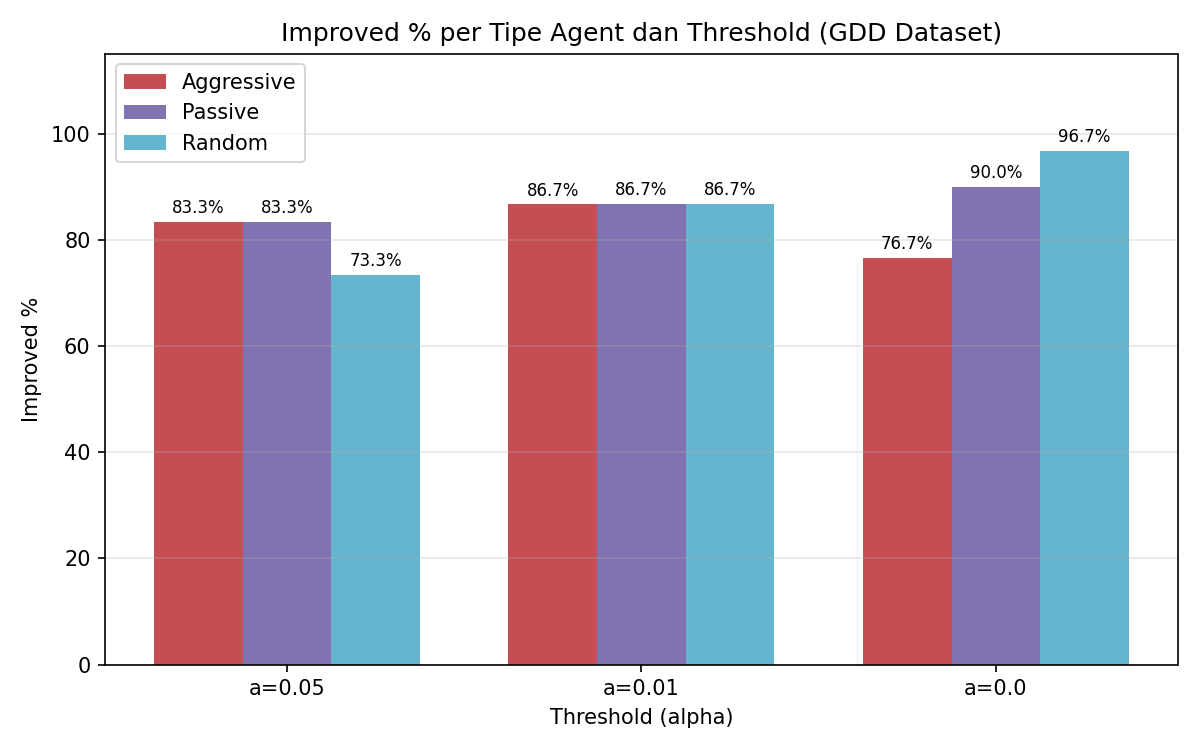
\includegraphics[width=0.75\textwidth]{tugas-akhir/assets/images/plot_per_agent.png}
    \caption{Perbandingan Distribusi Hasil per Profil Agen ($\alpha=0.05$)}
    \label{fig:per_agent_plot}
\end{figure}

Agen \textit{aggressive} secara konsisten menghasilkan performa terbaik dengan \textit{Balanced \%} 63.33\% dan konvergensi tercepat (median generasi 3.0). Hal ini disebabkan oleh interaksi agen agresif yang lebih sering memicu \textit{Converter} manual, menghasilkan aliran sumber daya yang lebih aktif dan sinyal fitness yang lebih kaya bagi algoritma evolusioner. Agen \textit{passive} dan \textit{random} menunjukkan \textit{Improved \%} yang sama dengan \textit{aggressive} (83.33\%) namun konvergensi lebih lambat (6.5 generasi), mencerminkan tantangan ekstra dari perilaku pemain yang lebih konservatif dan stokastik.

\subsection{Perbandingan dengan Penelitian Dasar}
\label{subsec:paper_comparison}

Tabel \ref{tab:paper_comparison} membandingkan hasil penelitian ini dengan hasil paper GEEvo asli \citep{Rupp_2024} sebagai referensi.

\begin{table}[htbp]
\centering
\caption{Perbandingan Hasil Penelitian dengan Paper GEEvo \citep{Rupp_2024}}
\label{tab:paper_comparison}
\begin{tabular}{lcccc}
\hline
\textbf{Sumber} & \textbf{Balanced \% ($\alpha$=0.05)} & \textbf{Balanced \% ($\alpha$=0.01)} & \textbf{Median Gen} & \textbf{Exec Time (s)} \\
\hline
Paper GEEvo (n=194)    & 93.3\%  & 83.0\% & 1.0   & 18.4   \\
TA — Abstrak (n=30)    & 66.67\% & 30.0\% & 2.5   & 1.191  \\
TA — MMORPG (n=10)     & 50.0\%  & 0.0\%  & 251.0 & 3.609  \\
TA — VHS/Horror (n=10) & 30.0\%  & 20.0\% & 500.0 & 18.004 \\
\hline
\end{tabular}
\end{table}

Perbedaan hasil dengan paper asli bersifat by design dan dapat dijelaskan oleh tiga faktor metodologis:
\begin{itemize}
    \item \textbf{Ukuran dataset}: Paper menggunakan $n = 194$ graf, sedangkan penelitian ini menggunakan $n = 30$ (abstrak) dan $n = 10$ (GDD), sehingga estimasi statistik kurang stabil dan rentan terhadap variasi sampel.
    \item \textbf{Kompleksitas topologi GDD}: Dataset MMORPG dan VHS memiliki topologi yang ditentukan dari konten dokumen nyata, yang tidak selalu memiliki karakteristik optimal untuk penyeimbangan cepat.
    \item \textbf{Penambahan simulasi agen}: Penggunaan \texttt{AgentSimulator} menambahkan lapis stokastisitas tambahan yang tidak ada pada paper asli, sehingga mempersulit konvergensi namun meningkatkan representasi pemain nyata.
\end{itemize}

Perbandingan ini bersifat \textit{referensial} — fokus utama evaluasi penelitian ini adalah perbandingan antar Kondisi A, B, dan C, bukan replikasi eksak paper asli. Tabel \ref{tab:paper_comparison} menunjukkan bahwa pada dataset abstrak ($n=30$), sistem TA mencapai \textit{Balanced \%} sebesar 66.67\% dengan waktu eksekusi rata-rata hanya 1.191 detik per graf, jauh lebih cepat dari paper (18.4 detik) meskipun dengan $\alpha$ yang sama.
